%%%%%%%%%%%%%%%%%%%%%%%%%%%%%%%%%%%%%%%%%%%%%%%%%
%%%%   SECTION 2b — LLM Augmented Generation %%%%
%%%%              (Phase 2)                  %%%%
%%%%%%%%%%%%%%%%%%%%%%%%%%%%%%%%%%%%%%%%%%%%%%%%%

\subsection{LLM Augmented Generation (Phase~2)}
\label{sec:phase2}
\subsubsection{Exercise}
Before proceeding with the development of the Retrieval-Augmented Generation system, we conducted three exercises to better understand how the positional and contextual embeddings, and self-attention as input embeddings go through the different layers.

\textbf{Positional Embeddings:} To analyze the structure of a BERT model's (MedCPT Query Encoder) positional embeddings, a sequence of 200 repetitions of the word "cat" was constructed and fed to the model. Since all tokens are identical (excluding CLS and SEP), the variation observed in the embeddings is only due to the differences in positional information related to where that token is in the input sentence (sequence information). For each token, the cosine distance to the first token was computed and illustrated in a graph with colour that encodes the distance value. As seen in the left of the Figure~\ref{fig:exercise_distances} below, the distance increases with token position, confirming that BERT's positional embeddings encode sequential order in a geometrically consistent manner, meaning that tokens that are closer in position are also closer in positional embedding space in a consistent way.

\begin{figure}[htbp]
  \centering
  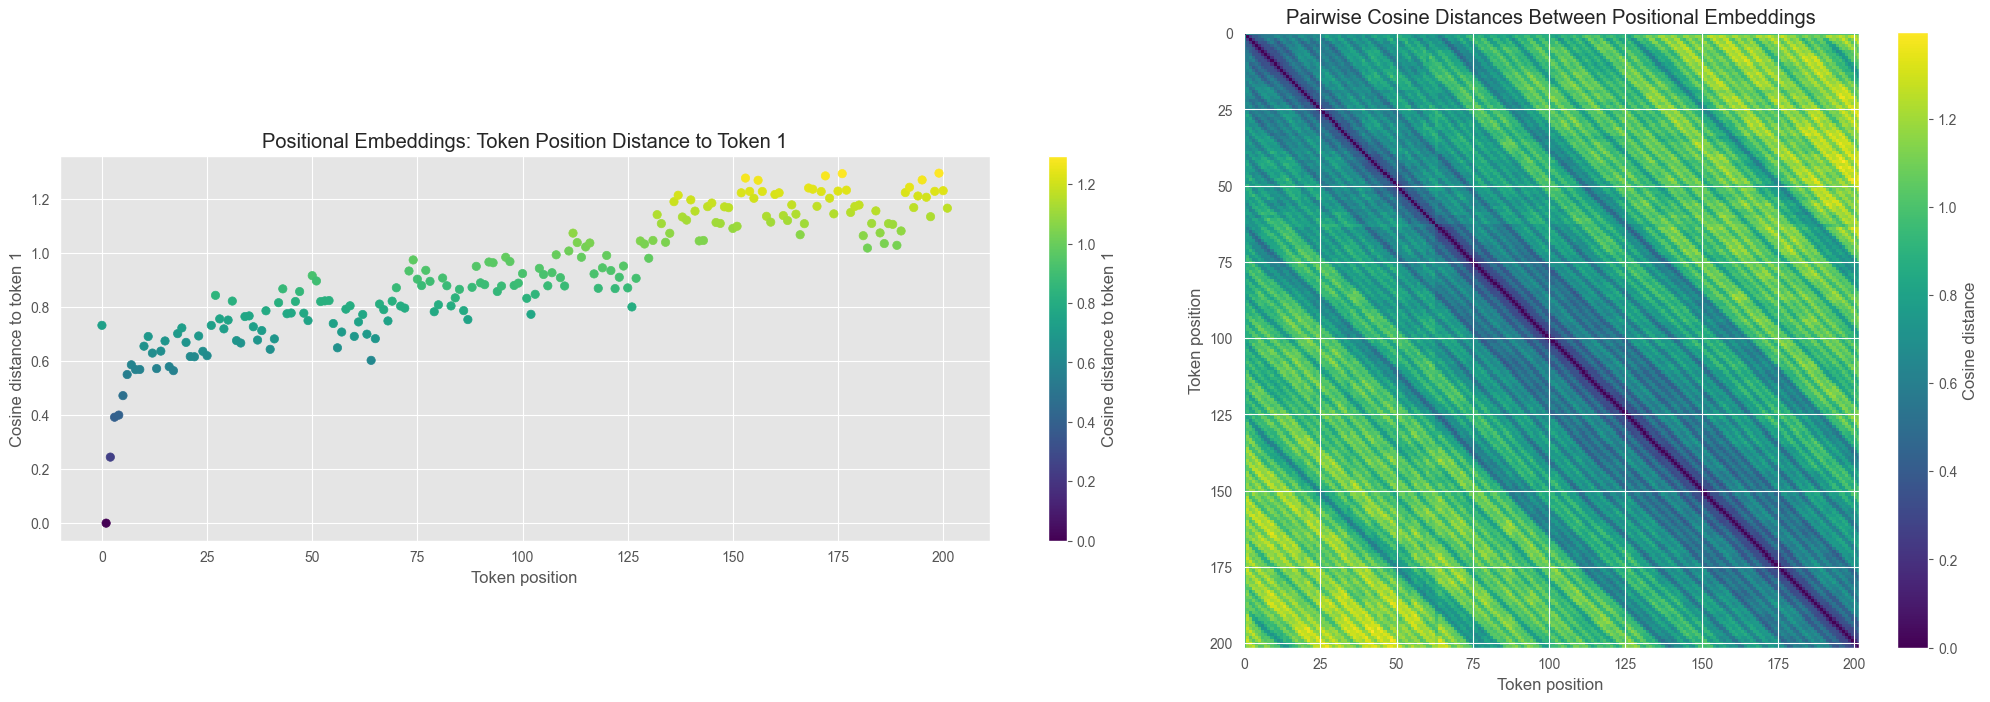
\includegraphics[width=\linewidth]{images/exercise_distances.png}
  \caption{Left: positional embeddings distances to the first "cat" token; Right: pairwise cosine distances between all tokens' positional embeddings}
  \label{fig:exercise_distances}
\end{figure}

Note that the CLS token has a cosine distance of 0.73 to the first token, which is normal since it is always fixed in position 0, due to the model also needing to learn a learn positional embedding for it. Its function is to serve as a summary token used in classification tasks.

This behaviour is further corroborated by the pairwise cosine distance matrix in the right of the previous Figure, which displays the distances between all pairs of token positions. It shows us a clear diagonal structure where entries closer to the main diagonal correspond to tokens closest in position and show low cosine distances (darker colour), while off-diagonal entries grow progressively larger as the positional gap between both tokens increase. This "banded" pattern confirms that positional similarity decays smoothly with distance, and that BERT's positional embeddings preserve a notion of local neighbourhood where nearby positions remain geometrically proximate in the embedding space.

\textbf{Contextual Embeddings:} To study how BERT models build contextualized semantic representations across layers, we extracted the output hidden states from all 12 layers and projected them into 2D/3D spaces with PCA.
Using the sentence "The cell membrane contains receptors. The receptor binds the ligand. Ligand binding activates the cell signaling pathway.", we observed that, in early layers, token representations form relatively "mixed" clusters with limited semantic relation. By layer 5, related tokens like "binds" and "binding" remain closer to each other in the embedding space, and are also closer to "receptor" than to less related concepts like "membrane" or "pathway". This behaviour is consistent with biomedical semantics, as binding interactions can be associated to receptor activity. In the final layers (of which the last can be seen in 3D in the Figure~\ref{fig:exercise_contextual}), the semantic organization becomes evident: signaling/activation tokens are closely related, and interaction-related concepts such as bindings and receptor interactions occupy a separate semantic region. Notably, the 2D projection placed "membrane" misleadingly close to these groups; the 3D projection revealed it is actually distant from both roughly at near the same distance/similarity with the SEP and "the" tokens, highlighting the limitations of 2D (first two eigenvalues) PCA appearing almost as far from them as from the isolated SEP and "the" tokens. The usage of the only first two eigenvalues made us lose that information (in 2D). Overall, this confirmed BERT progressively transforms lexical information into higher-level biomedical semantic structure across its layers.

\begin{figure}
    \centering
    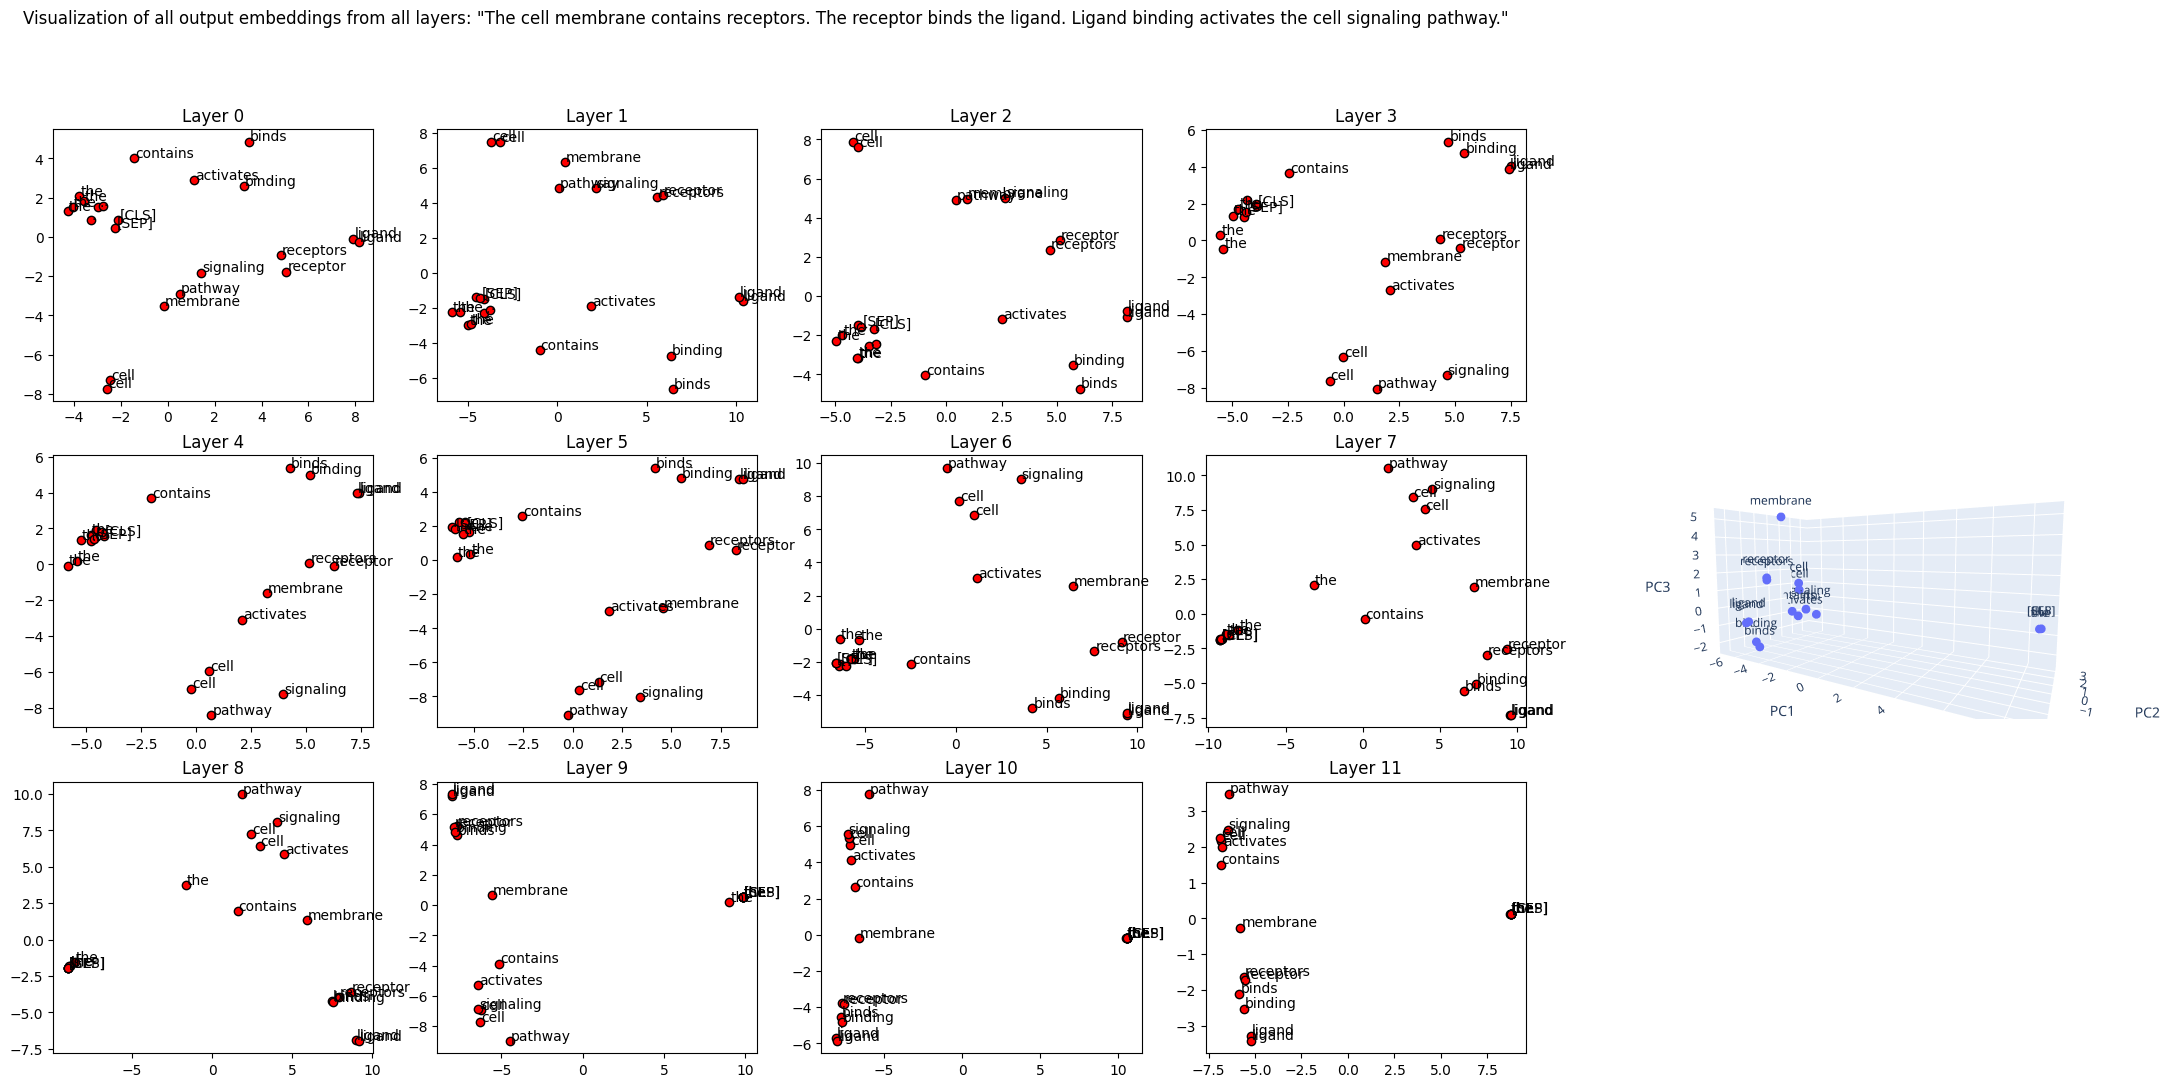
\includegraphics[width=\linewidth]{images/exercise_contextual.png}
    \caption{Left: 2D PCA projection of example contextual embeddings; Right: 3D PCA projection of example contextual embeddings}
    \label{fig:exercise_contextual}
\end{figure}

\textbf{Self-Attention:} For this exercise, we examined the self-attention mechanism of a transformer cross-encoder; in this case, MedCPT's Cross-Encoder.

One of the many examples we tested is the query "What drugs were prescribed to the patient with fever?" with answer "The patient was prescribed aspirin and ibuprofen to treat the fever.".

\begin{figure}
    \centering
    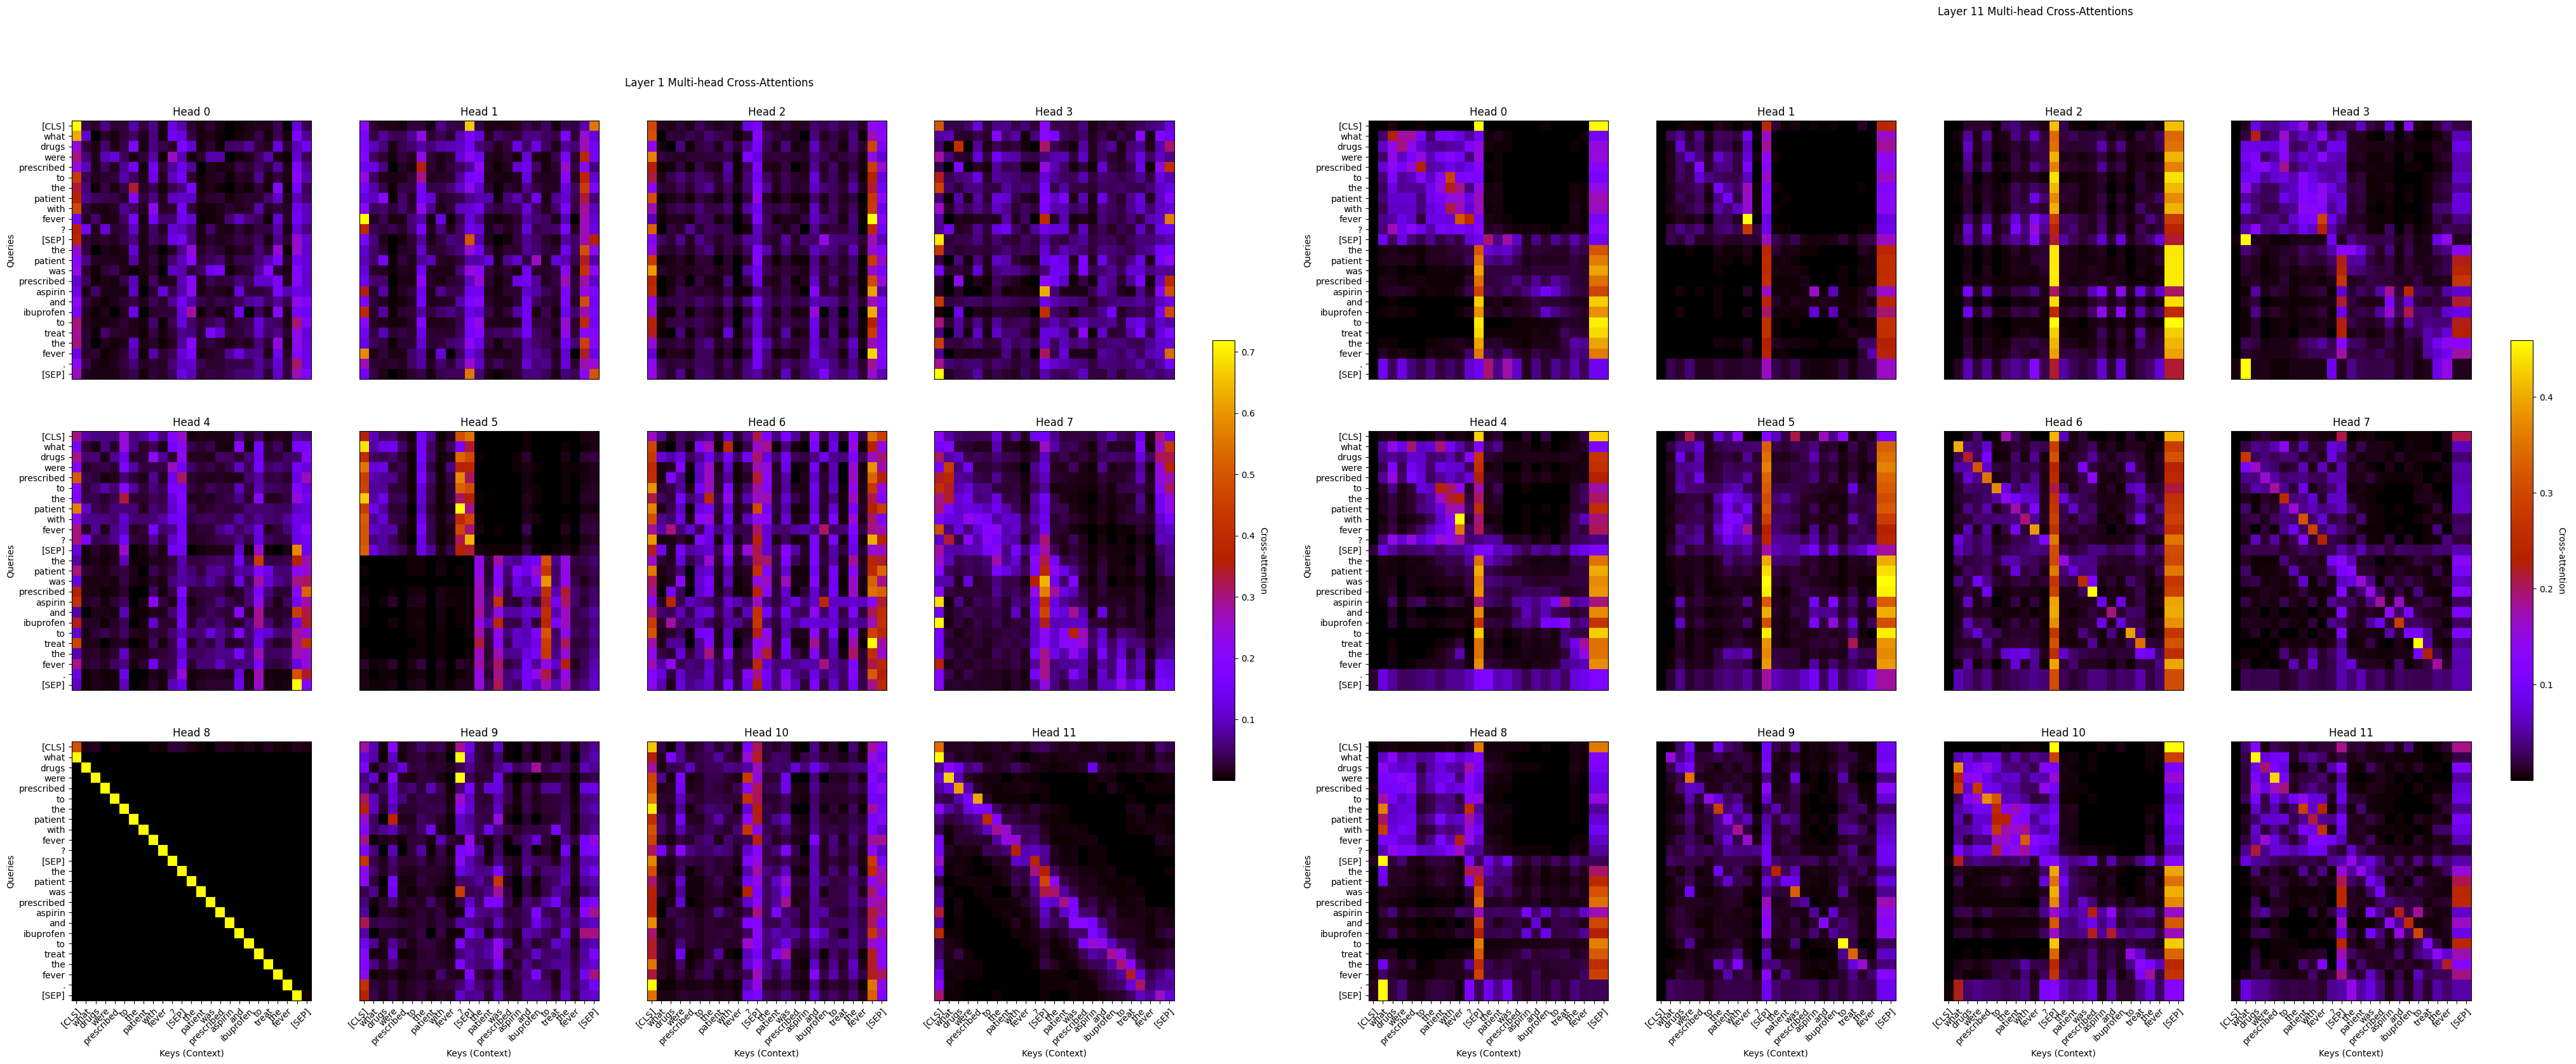
\includegraphics[width=\linewidth]{images/exercise_attention.png}
    \caption{Left: multi-head cross attentions for layer 1; Right: multi-head cross attentions for layer 11}
    \label{fig:exercise_attention}
\end{figure}

In this case, the layer one's attention heads tendentially focus more on local relations and basic syntatic dependencies, which can be seen in the high cross-attention values (brighter coloured) near the main diagonal of the matrices; these early attention heads tend to display more broad distributed attention. The final layer's attention heads attention values indicate a stronger and more specific cross-sentence attention; each head plays a specific, specialized role, allowing the model to better capture multiple perspectives on the input data. This is even more evident in the full visualization of all layers' multi-head self attentions in the Appendix~\ref{fig:model_view}.
Layer one shows a tendency of certain columns having a high attention score, but this is way more evident in the last layer, which illustrates the phenomenom of attention sink: the attention weights must sum to 1, but a token might not have a semantically meaningful target to attend to and it still has to place its probability mass somewhere; in this case, SEP becomes that "dump" token due to the fact that attending to it doesn't corrupt representations since its value vector is relatively uniformative, so routing attention there causes less damage than if it were done to other tokens.

\subsubsection{Answer Generation}
Phase 2 leverages the previous phase's results to extend the retrieval pipeline into a Retrieval-Augmented Generation system. To do this, we use MedCPT's Query Encoder to retrieve the index documents that best match a query, and then the Cross-Encoder reranker for sentence-level relevance scoring in order to get a well-built context to this specific query, that can be then passed to a decoder (Gemma 4 31B Instruction-Tuned) that generates a grounded answer with PMID citations.
Since the provided PubMed abstracts are plain text and are in the biomedical field, this requires a robust sentence boundary detection tool, rather than simple paragraph/period segmentation, in order to separate the abstracts into sentences. So, we analyzed (analytically) the difference between two different sentence segmentation libraries: NLTK and scispaCy.

\begin{table}[htbp]
\centering
\caption{NLTK vs. scispaCy comparison}
\label{tab:nltk_siscpacy}
\begin{tabular}{cccc}
  \hline
  \textbf{Property} & \textbf{NLTK} & \textbf{scispaCy} \\
  \hline
  Domain & General & Biomedical / Scientific Text \\
  Abbreviation Handling & Limited & Biomedical abbreviation-aware \\
  Basis & Statistics & Neural-Based \\
  Use Case & General NLP & Scientific Literature \\
  \hline
\end{tabular}
\end{table}

In theory, scispaCy should be much more appropriate for our use case, and this was also confirmed with the manual analysis of the sentence segmentation of 4 randomly selected corpus abstracts, and 1 handmade test. The handmade test is enough to understand why this sentence segmentation tool is the best choice (Fig.~\ref{fig:nltk_scispacy}):

\begin{figure}[htbp]
  \centering
  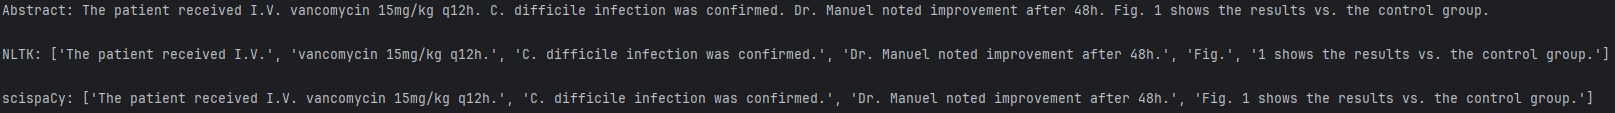
\includegraphics[width=\linewidth]{images/nltk_scispacy.png}
  \caption{NLTK vs. scispaCy: handmade test results}
  \label{fig:nltk_scispacy}
\end{figure}

scispaCy correctly identified abbreviations like "I.V." (intravenous) and preserved the sentence "The patient received I.V. vancomycin 15mg/kg q12h" as a single unit; NLTK incorrectly split it into two. This is critical when processing field-specific biomedical text like our dataset has. An additional example that further illustrate this difference is provided in the Appendix~\ref{fig:nltk_sciscpacy_ex2}.

After segmenting abstracts with sispaCy, we evaluated two sentence selection strategies over the top-10 retrieved documents (using MedCPT's Query Encoder). The first ranked all sentences from those documents by sorting the results of the MedCPT's Cross-Encoder, and then selected the top-10 sentences globally. The second enforced a per-document cap of 3 sentences before applying the same global top-10 selection.
Gemma 4 was then evaluated with a wide range of parameters (temperature, top-p, max sentences per document) and two different prompt templates using a frontier LLM as a Judge in order to identify the optimal setup for Phase 3. Varying the model parameters (temperature and top-p) allowed us to balance the model's output randomness by reshaping the probability distributions over the vocabulary, and restricting the set of candidate tokens, allowing us to assess whether a greater determinism improves answer quality. The two user prompt templates, in turn, explore whether providing the model with the full query context, topic, question and narrative, gives better results than only providing the context and question.